\chapter{Digitale Logica}
\label{chap:digitalelogica}

\subsection*{Introductie}
Deze week gaan we dieper in op de digitale logica die ten grondslag ligt van een CPU. We leren hoe we met basale componenten complexere circuits kunnen bouwen.  \\ \\
In het tweede deel gaan we bekijken hoe de architectuur van een simpele processor is opgebouwd. We maken kennis met zijn instructieset en bekijken o.a. hoe I/O aangestuurd kan worden.

\subsection*{Leerdoelen}
Na het bestuderen van dit hoofdstuk wordt verwacht dat je:
\begin{itemize}
    \item[--] weet wat de standaardlijst aan logische poorten zijn en hoe je die kunt gebruiken.
    \item[--] de wet van Moore kent
    \item[--] weet hoe enkele basis digitale schema's zoals, latches, flipflops, counters, registers en adders werken.
    \item[--] weet wat er bedoeld wordt met de kloksnelheid van een circuit.
    \item[--] weet je het verschil te benoemen tussen combinatorische en sequentiële logica.
    \item[--] weet wat een ALU is en waar de processor flags voor worden gebruikt.
    \item[--] weet wat een instructieset inhoudt van een CPU.
    \item[--] die instructies kunt indelen per categorie.
    \item[--] weet wat een interrupt is en hoe de CPU deze afhandelt.  
    \item[--] de verschillen kunt benoemen tussen memory-mapped en port-mapped I/O.
\end{itemize}

\subsection*{Relevant materiaal}

Bij dit hoofdstuk hoort hoofdstuk 2 \& 3 van het tekstboek van \textbf{Ledin}. (\href{https://learning.oreilly.com/library/view/modern-computer-architecture/9781803234519/Text/Chapter\_2.xhtml\#:-:text=2,Digital\%20Logic}{link}). 

\newpage
\section{Digitale logica}
Het basiscomponent waar zo'n beetje de hele CPU mee is opgebouwd is: de
transistor. We gaan zien hoe de transistor in de basis werkt, en hoe hiervan
simpele logische schakelingen mee te maken zijn.

\studeeraanwijzing{Bestudeer in \textbf{Ledin} de paragrafen \textit{Electrical circuits} t/m \textit{Latches} van hoofdstuk 2 (\href{https://learning.oreilly.com/library/view/modern-computer-architecture/9781803234519/Text/Chapter\_2.xhtml\#:-:text=We\%20begin\%20this\%20chapter\%20wit,es\%20of\%20electrical\%20circuits}{link}).}

\begin{opdracht}
  \begin{minipage}[t]{0.9\linewidth}
  \begin{enumerate}
      \item [A] Geef de waarheidstabel van een AND, en een OR.
      \item [B] Geef de waarheidstabel van een NAND, en een Negative-OR (een OR
        waarbij beide ingangen zijn geïnverteerd). Wat valt je op? 
      \item [C] Ga naar \href{https://logic.ly/demo}{logic.ly/demo} en simuleer
        een set-reset schakeling (\textit{Figure 2.10} uit \textbf{Ledin}). Gebruik als input voor
        $S$ en $R$ een \textit{Toggle Switch} en voor uitgang $Q$ een
        \textit{Light Bulb}. 
    \end{enumerate}
  \end{minipage}
\end{opdracht}

De simpele logische schakelingen die we net geleerd hebben, vormen weer de
basis voor complexere schakelingen. Schakelingen die bijv. reageren op
clocksignalen, (tijdelijk) gegevens kunnen opslaan of aritmische
berekeningen kunnen uitvoeren.

\studeeraanwijzing{Bestudeer in \textbf{Ledin} paragrafen \textit{Flip-flops} t/m \textit{Adders} van hoofdstuk 2 (\href{https://learning.oreilly.com/library/view/modern-computer-architecture/9781803234519/Text/Chapter\_2.xhtml\#:-:text=A\%20device\%20that\%20changes\%20its\%20output}{link}).}

\begin{opdracht}
  \begin{minipage}[t]{0.9\linewidth}
  \begin{enumerate}
        \item [A] Ga naar \href{https://logic.ly/demo}{logic.ly/demo} en simuleer een 4-bits (ripple carry) adder op basis van \textit{Figure 2.15}. Neem voor beide inputs $A$ en $B$, een groep van 4 \textit{Toggle Swichtes} en voor de output $S$ een groep van 5 \textit{Light Bulbs}.
        \item [B] Waarom is de output 1 bit groter dan de input?
    \end{enumerate}
  \end{minipage}
\end{opdracht}

Als de ingang van een logische schakeling veranderd, veranderd de uitgang
niet direct. Het duurt een fractie van een seconde om te veranderen, dit
noemen we \textit{propagation delay}. Het aan elkaar knopen van al die vele
componenten heeft daarom uiteraard invloed op het gehele systeem.  

\studeeraanwijzing{Bestudeer in \textbf{Ledin} \textit{Propagation delay} t/m \textit{Sequential logic} van hoofdstuk 2 (\href{https://learning.oreilly.com/library/view/modern-computer-architecture/9781803234519/Text/Chapter\_2.xhtml\#:-:text=When\%20the\%20input\%20of\%20a\%20logic\%20device\%20changes\%2C\%20the\%20output}{link}).}

\begin{opdracht}
  Is de \textit{SR Latch} uit \textit{Figure 2.10} een voorbeeld van sequentiële of combinatorische logica?
\end{opdracht}

\subsection{De wet van Moore}
De transistor, zoals je hierboven hebt gezien, is het fundamentele bouwsteentje van de moderne processor: een kleine schakelaar die stroom al dan niet doorlaat en zo een bit voorstelt. In de begindagen van de computer bestond een processor nog uit duizenden transistoren, terwijl een hedendaagse chip er miljarden bevat. Hoe kon die ontwikkeling zo razendsnel gaan?

In 1965 constateerde Gordon Moore, medeoprichter van Intel, een opvallend patroon: het aantal transistoren dat op een chip paste verdubbelde ruwweg elke twee jaar. Deze waarneming staat bekend als de \textbf{wet van Moore}. 
Het is geen natuurwet, maar een empirische voorspelling over de groei van de chipindustrie, die decennialang verrassend nauwkeurig is uitgekomen.

Figuur \ref{fig:moore-law} toont dit verloop. Let op de schaalverdeling van de verticale as: deze is zodanig gekozen dat de exponentiële groei over de jaren heen goed zichtbaar is. Elke sprong op de as betekent een verdoubling van het aantal transistoren per chip.

\studeeraanwijzing{Bestudeer in \textbf{Ledin} de paragraaf over ``Moore's law" (\href{https://learning.oreilly.com/library/view/modern-computer-architecture/9781803234519/Text/Chapter_1.xhtml#_idParaDest-24}{link}).}

\begin{figure}[h]
    \centering
    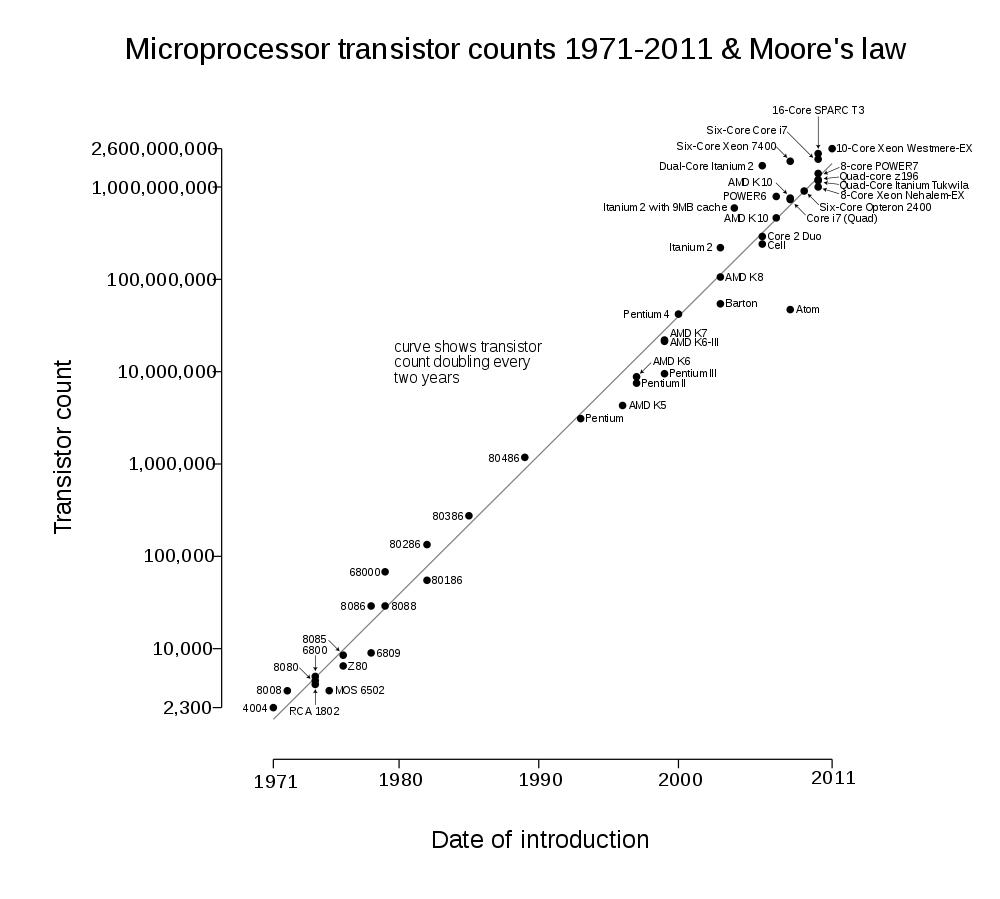
\includegraphics[width=\textwidth]{pictures/figuren/moore_law.png}
    \caption{De wet van Moore \\ {\small \textit{Wgsimon, CC BY-SA licentie}}}
    \label{fig:moore-law}
\end{figure}

% De wet van Moore is te zien in figuur \ref{fig:moore-law}. De schaalverdeling is aangepast op het verloop van de ontwikkelingen door de jaren heen. De figuur dient ter illustratie van de beschrijving in Ledin.

\newpage

\section{Processor elementen}

In dit stuk gaan we in op hoe een CPU globaal werkt, en wat z'n
voornaamste taken zijn. Dit doen we aan de hand van de \textit{6502}
processor, gezien z'n overzichtelijke structuur.

\studeeraanwijzing{Bestudeer in \textbf{Ledin} \textit{A simple processor} t/m \textit{Registers} van hoofdstuk 3. \\
  N.B.: Het stuk over VHDL kun je compleet overslaan. (\href{https://learning.oreilly.com/library/view/modern-computer-architecture/9781803234519/Text/Chapter\_3.xhtml\#:-:text=3,Processor\%20Elements}{link}).}

\begin{opdracht}
  \begin{minipage}[t]{0.9\linewidth}
  \begin{enumerate}
    \item [A] Geef een berekening waarbij de \textit{zero flag} ($Z$) hoog zou worden. 
    \item [B] Geef een berekingen waarbij de \textit{overlfow flag} ($V$) hoog zou worden.  
    \item [C] Benoem een voordeel van \textit{CISC} ten opzichte van \textit{RISC}. 
    \item [D] Benoem een voordeel van \textit{RISC} ten opzichte van \textit{CISC}. 
    \end{enumerate}
  \end{minipage}
\end{opdracht}

We gaan hier wat verder in op de instructieset van de CPU, en dan met
name in welke categorie\"en de instructies in te delen zijn.

\studeeraanwijzing{Bestudeer in \textbf{Ledin} paragrafen \textit{Instruction categories} t/m \textit{No operation instruction} van hoofdstuk 3 (\href{https://learning.oreilly.com/library/view/modern-computer-architecture/9781803234519/Text/Chapter\_3.xhtml\#:-:text=Instruction\%20categories,section\%20presents\%20the\%20categories}{link}).}

\begin{opdracht}
  Geef aan in welke cateregorie de volgende $6502$-instructies horen:
  \begin{lstlisting}
    LDA 
    CMP 
    DEX
    NOP
  \end{lstlisting}
  % Branch naar 'LABEL' als NUM1 >= NUM2.
\end{opdracht}

De processor kan (van buiten af) een verzoek om aandacht krijgen, dit noemen
we een \textit{interrupt}.

\studeeraanwijzing{Bestudeer in \textbf{Ledin} paragrafen \textit{Interrupt processing} t/m \textit{BRK instruction processing} van hoofdstuk 3 (\href{https://learning.oreilly.com/library/view/modern-computer-architecture/9781803234519/Text/Chapter\_3.xhtml\#:-:text=Interrupt-related\%20instructions\%20allow}{link}).}

\begin{opdracht}
  Geef 3 voorbeelden die je via een interrupt zou kunnen afhandelen.
\end{opdracht}

Ten slotte gaan we kijken naar de basis van I/O operaties, die gebruikt
worden om data over te brengen tussen de processor en de randapperatuur.

\studeeraanwijzing{Bestudeer in \textbf{Ledin} paragrafen \textit{Input/output operations} t/m \textit{Direct memory access} van hoofdstuk 3 (\href{https://learning.oreilly.com/library/view/modern-computer-architecture/9781803234519/Text/Chapter\_3.xhtml\#:-:text=Input\%2Foutput\%20operations,the\%20I\%2FO\%20portion}{link}).}

\begin{opdracht}
    Wat is het verschil tussen memory-mapped en port-mapped I/O?
\end{opdracht}
